\documentclass[10pt,a4paper]{report}
\usepackage{fancyhdr}
\usepackage{lastpage}
\usepackage{graphicx}
\graphicspath{{./images/}}

% Title Page
\title{Third Year Project Progress Report}
\date{18 November 2019}

\pagestyle{fancy}
\fancyhf{} % clear all fields

\fancyhead[R]{Toby Lawrance, 1731636, \thepage / \pageref{LastPage}}
\renewcommand{\headrulewidth}{0pt}

\begin{document}
\maketitle
\section*{Project Introduction/Specification}
	\subsection*{Statement}
		\subsubsection*{In Short:}
			Implementing Computer Vision algorithms to allow for robot navigation using the camera feed as the primary perception.
		\subsubsection*{Aims:}
			The aim of this project is to utilise the camera more efficiently as cameras are typically cheap sensors and this helps make robotics more affordable as a discipline, or at least to provide additional ways to aid internal sensor data and provide additional data points of belief in the robot's current pose.
		\subsubsection*{Objectives:}
			\begin{itemize}
				\item Move towards an object that is recognised in the environment. 
				\item Acknowledge obstacles in the environment and attempt to avoid them.
				\item Attempt to acknowledge more natural obstacles.
				\item Attempt to use the camera feed to aid with pose estimation.
			\end{itemize}
\section*{Progress made so far}
	\subsection*{ROS}
		\subsubsection*{Overview of the Robot Operating System}
			The Robot Operating System (ROS) is a meta-operating system that runs on top of a regular operating system. It is designed to be highly modular (though one could at times argue too modular) and typically run in a ``Publisher -> Subscriber" model, a unit of executable is referred to as a node and is typically recommended as a reusable task, for example ``sensor drive, sensor data conversion, obstacle recognition, motor drive, encoder input and navigation"\cite{pyo_ros_en_2017}
\section*{Future plans}
	\subsection*{Experiments}
		To test the effectiveness of the solution in a reasonably scientific way, a controlled environment is necessary. I'd like to create a simple maze environment for the robot to manoeuvre around. A number of arrangements for the maze can be generated. From this we can measure a number of parameters relating to the performance in moving through the environment. \\
		The format for the experiments will be thus: \\
		The robot will start on the edge of the environment facing towards the maze and from there attempt to find a red cube similar to this one: \\
		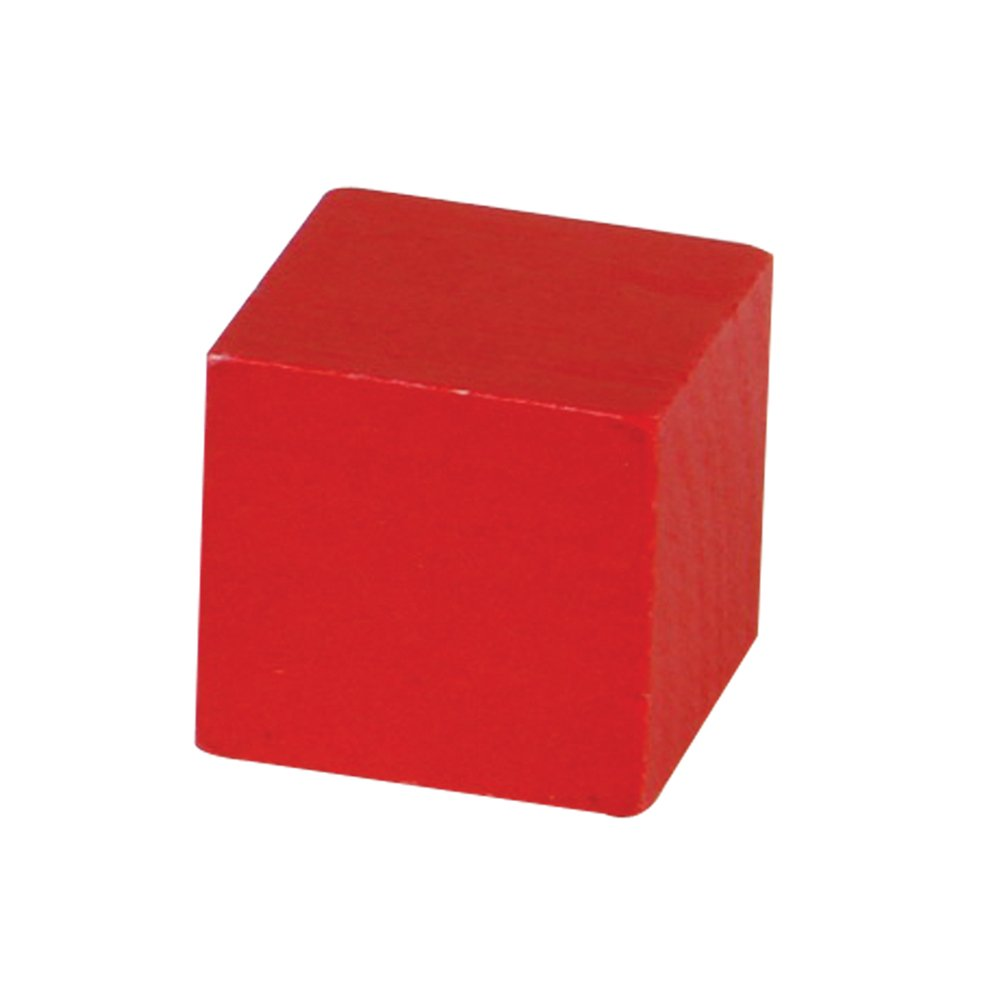
\includegraphics[scale=0.2]{RedCube}  \\
		This is simply to give the robot a reasonable chance of entering the environment and not immediately moving away from the environment which may result in a ``cheating" solution of going around the environment to find the target. \\
		For a given maze configuration these things can be measured about the maze:
		\begin{enumerate}
			\item Length of ideal route
			\item Number of obstacles in maze
			\item Size of maze
			\item Complexity of route as a measure of turns required to reach goal.
		\end{enumerate}
		Using this data to give a comparison between maze layouts, we can then measure a number of elements about the performance of a robot in this environment, such as:
		\begin{enumerate}
			\item Time to goal
			\item Obstacle collisions
			\item Wrong turns
			\item Battery power used
		\end{enumerate}
		These measurements can then provide comparisons between different stages of implementation. To provide a baseline, it may be worth implementing a simple ``Remote Control" program for the robot which provides a camera feed and simple control scheme to provide a benchmark against which the algorithm can be measured. This may also provide some aid in identifying bugs or issues in the setup.
	
	\subsection*{Resources to be used/acquired}
		These experiments will require a few resources to execute, thought they shouldn't be too difficult to acquire. 
		\begin{enumerate}
			\item Red cube
			\item Obstacles of small height, e.g. Non-red blocks
			\item Obstacles of robot-comparable height (Approx. 20cm)
		\end{enumerate}
		I am currently attempting to acquire the first two sets of items from an old toy left at home; this is proving only mildly difficult in terms of scheduling and distance. The third set of items I have yet to have any particularly good ideas for, although A4 sized folders (31cm x 28cm) are typically capable of standing on their own and would be a good height for this, as well as being generally cheap to buy if necessary, or I may be able to borrow enough.
		
	\subsection*{Implementation steps to take}
		The system is effectively split into two major parts: Vision analysis and robot control. Separately these two parts have progress to be made as well as integration to be done between them. A significant step is the use of a node for the ROS operating system made by another developer under the github handle ``klintan": (https://github.com/klintan/ros2\_usb\_camera) This node will hopefully enable some of the integration to be smoother by providing a cross point between the camera feed and the robot operating system. This saves the effort of having to implement such functionality manually thankfully. \\
		With this node in place, the live camera feed can be published to the controlling computer for processing and saving. Maintaining the robot - computer control balance seems to be in the spirit of ROS and enables greater processing power at the cost of latency which, given the robot’s maximum speed being fairly low, should hopefully not be problematic.
		\subsubsection*{Possible future stumbling blocks}
			This project like any other is not without some risks. The ROS system is genuinely a little bit frustrating but, given the progress that has been made so far, the project should have gotten over the largest hurdle of using the system. However, I cannot discount the possibility that some element of the system or understanding of its processes may cause a delay in the project. \\
			In regards to the computer vision, many of the algorithms that can be used to aid in this process are computationally expensive and reduce the effective update rate of the robot. Whilst millisecond by millisecond updates are not required, if the computation grows complex enough, there may be issues with the effective update rate growing too slow to move the robot at more than a snail's pace. Hopefully this can be mitigated with reduced resolutions and optimisation to the algorithm itself which may prove to be a benefit in improving the overall quality of the algorithm developed. \\
			There is a risk of the hardware failing in some way. The hardware has been very reliable thus far in the project and as such I do not consider this a particularly likely risk. Hardware projects have a habit of presenting various issues that distract from the main problem of the project. 
	\subsection*{Considerations for the presentation}
		Presenting this project should hopefully be quite interesting as far as demonstrations go. Two main methods of demonstrating come to mind: \\
		\begin{itemize}
			\item Live demonstration of maze solving with camera feed.
			\item Annotated video of robot solving the maze from camera feed showing identifications of obstacles and goal.
		\end{itemize}
		Having these two options gives a bit of leeway on how to present the project as the live demonstration may not necessarily be feasible given time and space constraints. However the annotated video should provide a reasonable backup that continues to be fairly interesting and show the capabilities of the project effectively. \\
		An ideal annotated video would show the robot moving through an environment with nicely drawn lines indicating belief in obstacle locations and approximate angles/distances away. This would give a frame by frame demonstration of the robot's capabilities in understanding its environment.
	

\section*{Management}

\bibliographystyle{plain}
\bibliography{ProgressReport}

\end{document}